\section{Module 86: Register Spilling}
\begin{flushright}
\textit{(scribed by Jai Javeria)}
\end{flushright}
What do we do when we do not get a valid k colouring for a graph. In such a case we need to save some registers in the memory and update our code accordingly.\\
\textbf{Note:} Graph colouring is a NP hard problem and we would generally use some heuristic to find a colouring.  It might be the case that there exist a k colouring for the graph but our heuristic is not able to find it. In this case also we would spill registers to the memory.\\
\subsection{Register Allocation with Spilling}
\begin{itemize}
    \item Try to colour the RIG with k colours (k=number of machine registers).
    \item If this is not possible, pick up a node as a candidate for spilling.
    \item This register will now live in memory. Remove the picked node and all of its incident edges from the RIG.
    \item Repeat until the graph becomes k colourable.
\end{itemize}
The idea behind this algorithm is that when we remove one node from the RIG, it becomes sparser and hopefully it would become k colourable now. The algorithm is guaranteed to work because in the worst case the RIG would become k colurable when it has only k nodes left.
\subsection{Which node to pick}
\begin{itemize}
    \item The main idea to pick the node is to make the graph sparser and thus k-colourable. So one could pick the node with the maximum edges. This would make the RIG most sparser one at a time and we can get our solution faster.
    \item But it could happen that the node we picked up represents a register value that is used extensively in the code. This variable should not be sent to live in the memory, otherwise the runtime memory accesses would increase. Thus a better alternative is to select a register which has the minimum static live range i.e. all the program points where it it live.
    \item But a variable used just in a loop would have a less static live range but if the loop runs a million times during runtime, it would be not good to store it in memory. Thus we could select registers to spill based on 'cold' regions, the regions which are not going to be executed many time during runtime, e.g. the initialization part of the code.
    \item But just looking at the code statically may not give an accurate picture of which regions are cold and hot. Thus often a combination of 2nd and the 3rd strategy is used for selecting nodes. A JIT (Just In Time) compiler has an advantage of determining cold and hot regions more accurately.
\end{itemize}
\subsection{Optimistic Colouring}
\begin{itemize}
    \item Pick a node to spill, say n, and remove it and its edges from the RIG.
    \item Colour the remaining graph with k colours ( by potentially spilling more nodes).
    \item After we have got a colouring, try to put n back into the graph such that we can find a colour for n too.
\end{itemize}
\subsection{Optimistic Colouring Example}
Lets take the RIG example from the previous module
\begin{center}
    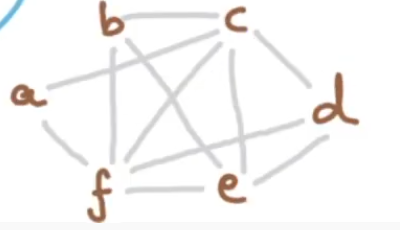
\includegraphics[scale=0.30]{images/85_RIGeg2.png}
\end{center}
And lets say we only have 3 registers for allocation and thus we need to find a 3 colouring. The current graph is not 3 colourable and thus we pick a node for spilling, say a.
\begin{center}
    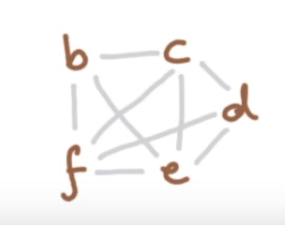
\includegraphics[scale=0.30]{images/86_remove_a.png}
\end{center}
We see that again the graph cannot be coloured in 3 colours and thus we select another node for spilling, say f. Now we can colour the graph with 3 colours.
\begin{center}
    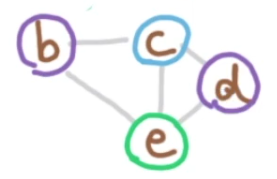
\includegraphics[scale=0.30]{images/86_color_RIG.png}
\end{center}
Now we try to add f back to the graph, but we cannot find a colour for f.
\begin{center}
    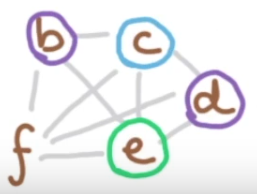
\includegraphics[scale=0.30]{images/86_add_f.png}
\end{center}
We move to adding a to the RIG and we are successful in colouring it.
\begin{center}
    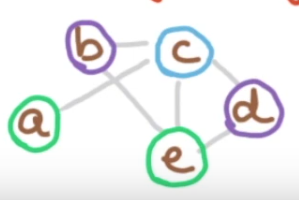
\includegraphics[scale=0.30]{images/86_add_a.png}
\end{center}
Thus finally we need to spill f to the memory.
\subsection{How to Spill}
\begin{itemize}
    \item Allocate a memory location for f on the stack frame. Let its address be $f_a$
    \item Before each operation that reads f, insert
        \begin{center}
            f = load $f_a$
        \end{center}
    \item After each write operation on f, insert
        \begin{center}
            store f, $f_a$
        \end{center}
    \item Also rename every use of f to f1,f2... . This would be beneficial for some further analysis that needs to be done. Since each different instance of f would be getting different values, it is possible to rename them to different variables.
\end{itemize}
\subsection{Effect of Spilling on RIG}
Since we have broken down f into different variables with short live ranges, the graph becomes sparser and easier to colour.
